% intro

ML have many applications in experimental particle physics like event identification and reconstruction which is the main focus of this thesis work.
Before going into detail of using ML in calorimeter cluster calibration we are going to introduce some background information related to the used ML methods in this work.%(Check this source for more info and source).

Before talking about ML, we need to introduce Artificial intelligence (AI).
AI is the process of computers being trained to imitate how the human brain learns and solves problems. An AI computer program,
software, could be simple as a chess game or complex as one that can predict the RNA structure of a virus to help develop vaccinee% source1.
There are different types of AI, as shown in the related figure, ML is a subsection of AI and DL is a subsection of ML.
To understand the difference between ML and DL, ML is of AI where it needs a human intervene to improve its learning and DL where computers learn from its own past mistakes.
%(Source for more info about deep learning.)  

When talking about ML there are few concepts want need to be explained. Starting with AI algorithm which means the programming,
a set of instructions, that tells the computer how to learn to operate on its own source2 to solve a problem or do a task.
ML models are computer programs used to recognize patterns in data (classification) or make predictions (regression) in other words they are the output of the training the ML algorithm using training data.
To summarize this ML models are created using ML algorithms that undergo a training process with a data to modified the algorithm to be better at manage the specific task and becomes a ML model.  %Source3

ML algo could be categorized into three main groups depending on type of data used in the training process: supervised learning, unsupervised learning, reinforcement learning.
as seen (in figure related) data could be labeled, unlabeled. Labeled data is any data the has an attribute or category assigned to for example like the price of a product or the Hight or a human.
For ML, Various python-based libraries such as schitkit-learn, TensorFlow, keras are used tools for ML algorithms and model implementation. 

In this chapter will describe one of the most commonly used ML algorithms in HEP (source):  boosted Decision trees and Neural networks.  


\begin{figure}[t!]
\centering
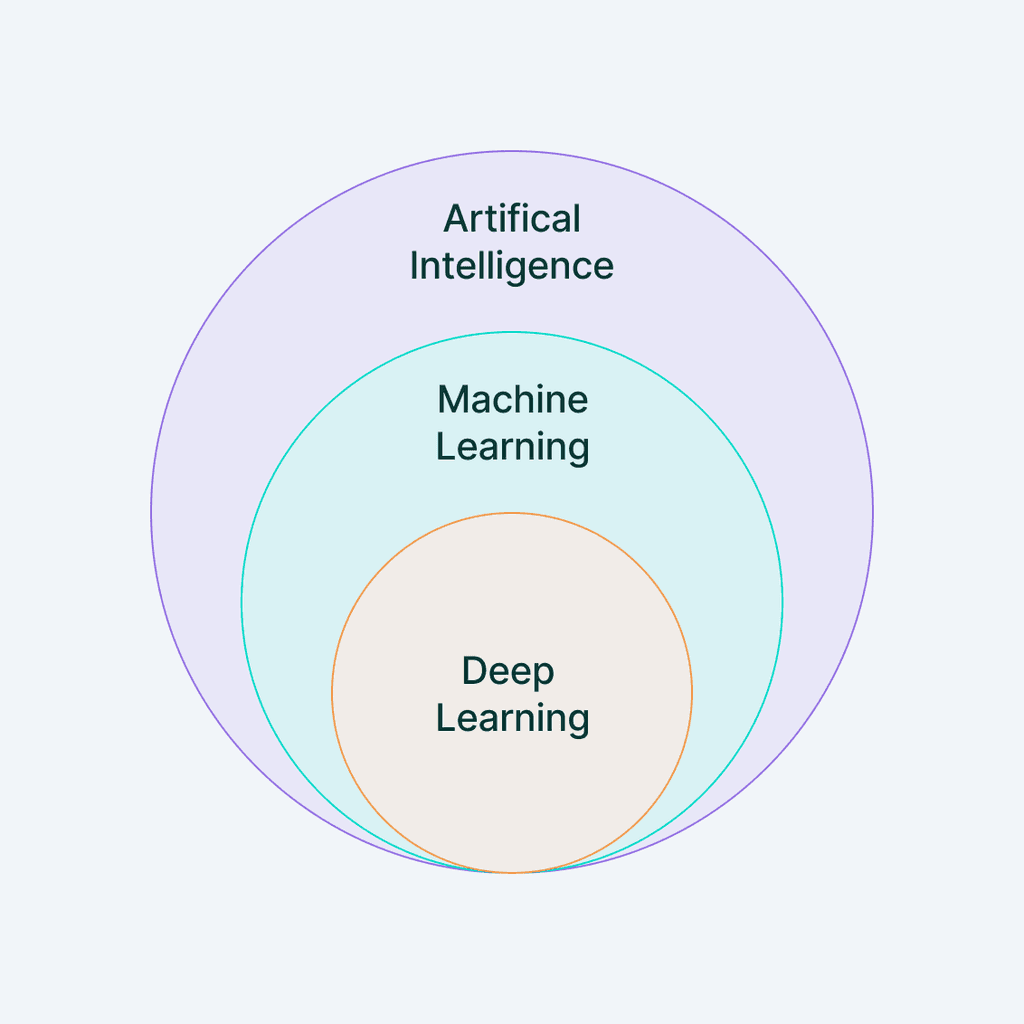
\includegraphics[width=0.99\textwidth]{figures/ML_diagram.png}
\caption[ML and AI]{}. Figure source~\cite{SMtable}.
\label{fig:ML_diagram}}                                                                                                                                                                                        
\end{figure}
  
\section{BDT}

A decision trees (DT) is a type of algorithm that looks like an upside-down tree that starts with a root and then branches out to leaves. A DT has different level of nodes: Root node: top most node and it represent the entire message of the decision.
Decision node: a node where the prior node branches into two or more. leaf node: it is the last node in DT and there furthers from the root node. DTs are supervised learning algorithms where they can be used to make classification and regression models (this thesis deal with regression problems,  

In DT each node the split is chosen to maximalize the information gain (difference between in entropy before and after the potential split) in other words minimizing the entropy.
Entropy is max for 50/50 split and mini for 1/0 split. The spilt is created reclusively (iteratively) and this process is repeated until some stop condition is met. (ex: depth of tree no more information gains etc).

DT boosting uses a boosting technique that iteratively works to improve the weak trees by combining more that will correct the error of the previous one.
Meaning that the new tree will be trained on the samples that were misclassified by the previous model which gradually will refine the overall accuracy.
in other words, the final prediction is the weighted average of all models with more weight given to those with higher accuracy.
%(double check this sentence)  

There are different ways to iteratively adding learners to minimize a loss function most common ones for example are Adaboost (adaptive boosting), Gradient boosting, XGBoost (which will be used later for ECAL CAL).

\section{NN} 

Neural Networks (NN), also called artificial neural networks because of how they mimic the neurons in the brain sending signals to each other.
They are one of the most used ML algorithms (in particle physics).
The simplest NN contains an input, output, one hidden layer each containing number of neurons that are connected. NN are the backbone of deep learning algo if they have more one hidden layer. (insert picture of NN with multiple layers) 

NN like other DL algorithms relay on training data to learn to improve its accuracy overtime without human intervention.
They are many types of NN but most of them are feedforward (meaning they only flow in one direction from input to output, or called multiple layer perceptron's (MLP’s)).
Am mentioned before each layer have multiple neurons and each one of those neurons could think of it as its one linear regression model (expand more here) that contain input data (features?), weights, bias (threshold?) and output.

(insert here formula) weight help determine the importance of any given variable (features).
All inputs then multiplied by their respective weights and then summed.
Afterward the output is passed through the activation function (which determines the output) if the output exceeds a given threshold, it activates the node and passing data to the next layer in the network.
This results in the output of one node becoming in the input of the next node.
This process of passing data from one layer to the next layer defines this NN as feedback network.
(we can get into depth of how the NN are trained).
The goal is minimizing the cost/loss function.to insure the fitting of the model. As the model adjusts its weight and bias. Until reaches a local minimum. 






